\section{Problem definition and modeling}
In this section, we explain the general architecture of DNN layers and our profiling method. Moreover, we elaborate on how the cost optimization can be reduced to a shortest path problem by introducing the JointDNN graph model. Finally, we show how the constrained problem is formulated by setting up ILP. 

\subsection{DNN Building Blocks}
DNNs are networks composed of several layers stacked to each other. We briefly explain the functionality of each layers used in the state-of-the-art architectures: 

\textbf{Convolution Layer} \textit{(conv)} consists of a set of filters with dimensions relatively smaller than their input. Each filter completely traverses through the input with a predefined step size and computes the dot product between it's parameters and the corresponding part of the input. This process creates different feature maps (referred to as channels) for different filters from the same input data. This aspect of preserving the locality of input features has made Convolutional Neural Network (CNN) architectures the horse power of the state-of-the-art image classification models. Because of dot product basis of \textit{conv}, it can be formulated as General Matrix Multiplication (GEMM), therefore capable of gaining performance improvement by using parallel computing devices (e.g. GPUs). 

\textbf{Fully Connected Layer} \textit{(fc)} is the main component of most regular neural networks in which every neuron is connected to all neurons of the previous layer. This fully pairwise connection architecture comprises large portion of computation of the whole network. Like \textit{conv}, \textit{fc} layer is also formulated as GEMM. 

% TODO: Major task of pooling: increasing the receptive field
\textbf{Pooling Layer} \textit{(pool)} performs a non-linear down sampling function over non-overlapping spatially local parts of input. Max-pooling is the most common function used in this type of layer alongside other functions such as average or L2-norm pooling. 

\textbf{Activation Layer} increases the non-linearity property of neural network architectures. This layer applies non-linear activation function on single data points of input to generate an output with the same size. Among various non-linear functions, such as sigmoid and hyperbolic tangent, Rectified Linear Unit \textit{(relu)} is currently the favorable choice in DNN architectures as it is simple and speeds up the tedious training process~\cite{ReLUpaper}. 

\textbf{Local Response Normalization} \textit{(lrn)} performs local normalization by imposing a local competition for big activities between adjacent features in a channel, and also between features at the same spatial location in different channels. \textit{lrn} are inspired by inhibition schemes observed in the brain helps with intention of generalization. There are different formulations suggested for \textit{lrn}, as shown in~\cite{AlexNet, multiStageArc} they may lead to slight improvements. 

% TODO: Consider p as probability of keeping the neuron active in training. During testing all neurons are present but their outputs are multiplied by p to maintain the scale of inputs. Add this to paper! 
\textbf{Dropout Layer} \textit{(drop)} 
As mentioned earlier, \textit{fc} occupies most of the parameters of DNN models and thus vulnerable to overfitting. Typically regularization methods are used to prevent overfitting by reducing high dependency of network on individual neurons during training. In dropout~\cite{DropOut} technique, at each training iteration every neurons can be removed (droped out) from network with a predetermined probability $p$ or kept with probability $1-p$ and the training is done on the remaining network. The dropped out nodes will have their previous weight for the next training iteration. 

\textbf{Deconvolution Layer} \textit{(deconv)} also known as transposed convolution is mostly used on generative and autoencoder models in applications such as building high-resolutions picture from low-resolution pictures and high-level descriptions. The goal in deconvolution is to find $f$ in the convolution equation of form $f*g=h$. In case of DNNs, $g$ is the filter and $f$ is the input of the convolution~\cite{Deconv}.

\textbf{Long Short-Term Memory Layer} \textit{(lstm)} is a building unit for layers of a recurrent neural network (RNN) and is widely used due to its promising results in speech recognition applications. A typical LSTM unit is composed of a cell, an input gate, an output gate and a forget gate, which is responsible for remembering and forgetting specific values over arbitrary time intervals. The whole LSTM unit can be thought as a typical artificial neuron, as in a feed-forward neural network.

\textbf{Softmax} \textit{(soft)} is the last layer in multi-class architectures, usually connected in a one-to-one correspondence way to a \textit{fc} layer. Softmax establishes a probability distribution by representing each class probability with a single neuron. 

% \begin{itemize}
% \item basic idea explained again: each node can be calculated either in mobile or cloud. Computation time on mobile, computation time on server, energy(power), P mobile, P cloud and comm. time.
% \item consecutive layers, explained in details in \textbf{ref 2 Experiments}. 
% \item The time of the communication is related to 1. amount of the data at the output of the layer \textbf{ref 2 Compression},  communication specifications \textbf{ref to communication spec}. 

% \item graph representation of the problem
% \item modeling of inference into graph
% \item modeling of training into graph
% \item reducing the problem to the shortest path problem, explaining the shortest path problem (complexity, etc. maybe here, implementation of the algorithm in results section)
% \item we will explain each DNN structure later \textbf{ref to different DNN structures} but here we should note that modeling the graph in some DNN (resNet) is more complicated and explained later. 
% \item What about constraints? They make this problem NP, \textbf{TODO:} possibly using ILP.

% \end{itemize}

\subsection{Energy and Latency Profiling}
\label{energy_latency_profiling}
There are three methods in measuring the latency and energy consumption of each layer in neural networks: 

\textbf{Statistical Modeling:} In this method, a regression model over the configurable parameters of operators (e.g. filter size in convolution) can be used to estimate the associated latency and energy. This method is prone to large error because of the inter-layer optimizations performed by DNN software packages. Therefore, it is necessary to consider execution of several consecutive operators grouped with each other during profiling. Many of these software packages are proprietary, making access to inter-layer optimization techniques impossible. 

% NVIDIA\textsuperscript{\textregistered} 

In order to illustrate this issue, we designed two experiments with 25 consecutive convolutions on NVIDIA Pascal\textsuperscript{\texttrademark} GPU using cuDNN\textsuperscript{\textregistered} library~\cite{cuDNN}. In the first experiment, we measure the latency of each convolution operator separately and set the total latency as sum of them. In the second experiment, we group the convolutions together and measure the total latency. All parameters are located on GPU's memory in both experiments, avoiding any data transfer from the main memory to make sure results are exactly representing the actual computation latency. 

% ALLIGN!

As we see in Figure~\ref{grouped_execution}, there is a large error gap between separated and grouped execution experiments which grows as the number of convolutions is increased. This observation confirms that we need to profile grouped operators to have more accurate estimations. Considering various consecutive combination of operators and different input sizes, this method requires a very large number of measurements, not to mention the need for a complex regression model.

% TODO: Erfan: Change it to layer count! Change the explanation! 
\begin{figure}
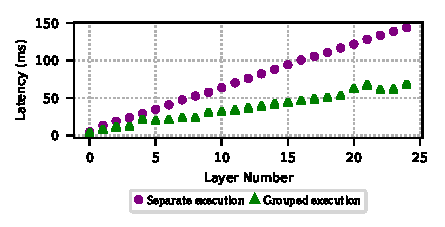
\includegraphics{consec}
\caption{Latency of grouped and separated execution of convolution operator.}\label{grouped_execution}
\end{figure}

\textbf{Analytical Modeling:} To derive an analytical approach for estimation of the latency and energy consumption, it is required to obtain the exact hardware and software specifications. However, the state-of-the-art work in latency modeling of DNNs~\cite{Paleo} fails to estimate layer-level delay within an acceptable error bound, for instance, underestimating the latency of a fully connected layer with 4096 neurons by around 900\%. Industrial developers do not reveal the detailed hardware architecture specifications and the proprietary parallel computing architectures such as CUDA\textsuperscript{\textregistered}, therefore, analytical approach could be quite challenging~\cite{GPUMODEL}.

\textbf{Application-specific Profiling:} In this method, the DNN architecture of the application being used is profiled in run-time. The number of applications in a mobile device using neural networks are generally limited. In conclusion, this method is more feasible, promising higher accuracy estimations. We have chosen this method for estimation of energies and latencies in the experiments of this paper. % HERE!

\subsection{JointDNN Graph Model}
First, we assume that a DNN is presented by a sequence of distinct layers with a linear topology as depicted in Figure~\ref{linear_topology}. Layers are executed sequentially, with output data generated by one layer feeds into the input of the next one. We denote the input and output data sizes of k$^{th}$ layer as $\alpha_k$ and $\beta_k$, respectively. Denoting the latency (energy) of layer k as $\omega_k$, where $k = 1, 2, ..., n$, the total latency (energy) of querying the DNN is $\sum_{k=1}^{n}{\omega_k}$.

% k$^{th}$

The mobile cloud computing optimal scheduling problem can be reduced to a shortest path problem, from node $S$ to $F$, in the graph of Figure~\ref{linear_topology_mc}. \textbf{Mobile Execution} cost of the k$^{th}$ layer ($C(ME_k)$) is the cost of executing the k$^{th}$ layer in the mobile while the cloud server is idle. \textbf{Cloud Execution} cost of the k$^{th}$ layer ($C(CE_k)$) is the executing cost of the k$^{th}$ layer in the cloud server while the mobile is idle. \textbf{Uploading the Input Data} cost of the k$^{th}$ layer is the cost of uploading output data of the (k-1)$^{th}$ layer to the cloud server $(UID_k)$. \textbf{Downloading the Input Data} cost of the k$^{th}$ layer is the cost of downloading output data of the (k-1)$^{th}$ layer to the mobile $(DID_k)$. The costs can refer to either latency or energy. However, as we showed in Section~\ref{energy_latency_profiling}, the assumption of linear topology in DNNs is not true and we need to consider all the consecutive grouping of the layers in the network. This fact suggests replacement of linear topology by a tournament graph as depicted in Figure~\ref{packing_topology}. We define the parameters of this new graph, \textit{JointDNN graph model}, in Table~\ref{jointDNNGraphParam}. 

\begin{figure}[t]
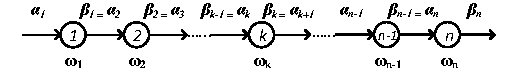
\includegraphics{linear_topology}
\caption{Computation model in linear topology.}\label{linear_topology}
\end{figure}

\begin{figure}[t]
%\includegraphics[height=1in, width=1in]{fly}
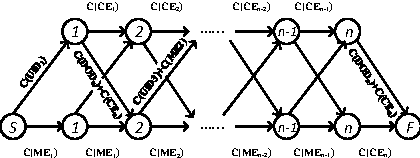
\includegraphics{linear_topology_mc}
\caption{Graph representation of mobile cloud computing optimal scheduling problem for linear topology.}
\label{linear_topology_mc}
\end{figure}


\begin{table}[b]
\caption{Parameter Definition of Graph Model} % title of Table
\label{nonlin_inputs} % is used to refer this table in the text
\centering % used for centering table
\begin{tabular}{|c|c|} % centered columns (4 columns)
\hline %inserts double horizontal lines
\textbf{Param.} & \textbf{Description of Cost}\\ [0.5ex] % inserts table
%heading
\hline % inserts single horizontal line
$CE_{i:j}$ & Executing layers $i$ to $j$ on the cloud \\
\hline % inserts single horizontal line
$ME_{i:j}$ & Executing layers $i$ to $j$ on the mobile \\
\hline % inserts single horizontal line
$ED_{i,j}$ & $CE_{i:j}$ + $DID_j$\\
\hline % inserts single horizontal line
$EU_{i,j}$ & $ME_{i:j}$ + $UID_j$\\
\hline % inserts single horizontal line
$\phi_{k}$ & All the following edges: $\forall i=1:k-1$ $ED_{i,k-1}$\\
\hline % inserts single horizontal line
$\Omega_{k}$ & All the following edges: $\forall i=1:k-1$ $ME_{i,k-1}$\\
\hline % inserts single horizontal line
$\Psi_{k}$ & All the following edges: $\forall i=1:k-1$ $EU_{i,k-1}$\\
\hline % inserts single horizontal line
$\Gamma_{k}$ &  All the following edges: $\forall i=1:k-1$ $CE_{i,k-1}$\\
\hline % inserts single horizontal line
$\Pi_m$ & All the following edges: $\forall i=1:n$ $ME_{i,n}$\\
\hline % inserts single horizontal line
$\Pi_c$ & All the following edges: $\forall i=1:n$ $ED_{i,n}$\\
\hline % inserts single horizontal line
$U_1$ & Uploading the input of the first layer\\
\hline %inserts single line
\end{tabular}
\label{jointDNNGraphParam}
\end{table}

\begin{figure*}
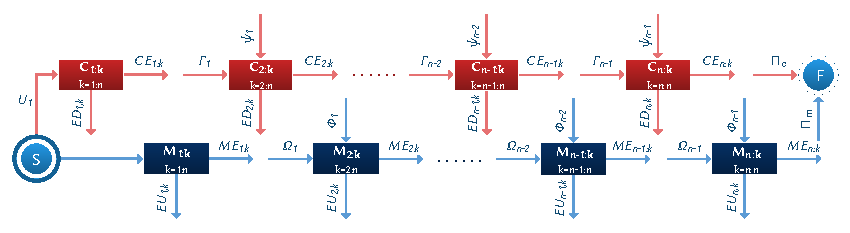
\includegraphics{packing_topology}
\caption{JointDNN graph model.}
\label{packing_topology}
\end{figure*}

% We introduce two dummy nodes: node S as the starting node and node F as the finishing node. 

% the k$^{th}$ layer

In this graph, node $C_{i:j}$ represents that the layers $i$ to $j$ are computed on the cloud server, while node $M_{i:j}$ represents that the layers $i$ to $j$ are computed on the mobile device. An edge between two adjacent nodes in JointDNN graph model is associated with four possible cases: 1) A transition from the mobile to the mobile, which only includes the mobile computation cost ($ME_{i,j}$) 2) A transition from the cloud to the cloud, which only includes the cloud computation cost ($CE_{i,j}$) 3) A transition from the mobile to the cloud, which includes the mobile computation cost and uploading cost of the inputs of the next node ($EU_{i,j} = ME_{i,j} + UID_{j+1}$) 4) A transition from the cloud to the mobile, which includes the cloud computation cost and downloading cost of the inputs of the next node ($ED_{i,j} = CE_{i,j} + DID_{j+1}$). Under this formulation, we can transform the computation scheduling problem to finding the shortest path from $S$ to $F$. 

Residual networks are a class of powerful and easy-to-train architectures of DNNs~\cite{ResNet}. 


In residual networks, as depicted in Figure~\ref{resnet} (a), the output of one layer is fed into another layer with distance of at least two. Thus, we need to keep track of the source layer (node $2$ in Figure~\ref{resnet}) so as to know that this layer is computed on the mobile or the cloud. 

Our standard graph model has a memory of one which is the very previous layer. We provide a method to transform the computation graph of this type of network to our standard model, JointDNN graph. 

In this regard, we add two additional chains of size $k-1$, where $k$ is the number of nodes in the residual block ($3$ in Figure~\ref{resnet}). One chain represents the case of computing layer $2$ on the mobile and the other one represents the case of computing layer $2$ on the cloud. In Figure~\ref{resnet}, we have only shown the weights that need to be modified, where $D_2$ and $U_2$ are the cost of downloading and uploading the output of layer $2$, respectively.

By solving the shortest path problem in JointDNN graph model, we can obtain the optimal scheduling of inference in DNNs. Online training consists of one inference and one back-propagation step. The total number of layers is noted by $N$ consistently throughout this paper so there are $2N$ layers for modeling training, where the second $N$ layers are the mirrored version of the first $N$ layers, and their associated operations are the gradients of the error function with respect to the DNN's weights. The main difference between the mobile cloud computing graph of inference and online training is the need for updating the model by downloading the new weights from the cloud. We assume that the cloud server performs the whole back-propagation step separately, even if it is scheduled to be done on the mobile, therefore, there is no need for mobile device to upload the weights that are updated by itself in order to save mobile energy consumption. The modification in JointDNN graph model is adding the costs of downloading weights of the layers that are updated in the cloud to $ED_{i,j}$.

The shortest path problem can be solved in polynomial time efficiently. 

However, the problem of shortest path subjected to constraints has been shown to be NP-Complete~\cite{NPComplete}. For instance, assuming our standard graph is constructed for energy and we need to find the shortest path subject to the constraint of the total latency of that path being less than a time deadline (QoS). However, there is an approximation solution to this problem, "LARAC" algorithm~\cite{LARAC}, the nature of our application does not require to solve this optimization problem frequently, therefore, we aim to obtain the optimal solution. We can constitute a small look-up table of optimization results for different set of parameters (e.g. network bandwidth, cloud server load, etc.). We provide the ILP formulations of DNN partitioning in the following sections.

\begin{figure}[b]
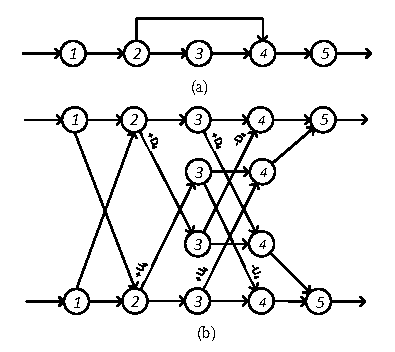
\includegraphics{resnet}
\caption{(a) A residual building block (b) Transformation of a residual building block into shortest path problem.}\label{resnet}
\end{figure}

\subsection{ILP Setup}

\subsubsection{Performance Efficient Computation Offloading ILP Setup for Inference}

We formulated the scheduling of inference in DNNs as an ILP with tractable number of variables. In our method, first we profile the delay and energy consumption of consecutive layers of size $m$ $\in$ $\{1, 2,\dots, N\}$. Thus, we will have
  \begin{equation}
      \begin{split}
N + (N-1) + ... + 1 = N(N+1)/2
  \end{split}
\end{equation}
number of different profiling values for delay and energy.
Considering layer $i$ to layer $j$ to be computed either on the mobile device or cloud server, we assign two binary variables $m_{i,j}$ and $c_{i,j}$, respectively. Download and upload communication delays needs to be added to the execution time, when switching from/to cloud to/from mobile, respectively.

\begin{equation}
      \begin{split}
T_{computation} &= \sum_{i=1}^{n}{\sum_{j=i}^{n}{
(m_{i,j}.T_{mobile_{L_{i,j}}} + c_{i,j}.T_{cloud_{L_{i,j}}})
}}
  \end{split}
\end{equation}
  \begin{equation}
      \begin{split}
T_{communication} &= \sum_{i=1}^{n}{\sum_{j=i}^{n}{\sum_{k=j+1}^{n}{m_{i,j}.c_{j+1,k}.T_{upload_{L_j}}}}} \\
& + \sum_{i=1}^{n}{\sum_{j=i}^{n}{\sum_{k=j+1}^{n}{c_{i,j}.m_{j+1,k}.T_{download_{L_j}}}}} \\
& + \sum_{i=1}^{n}{c_{1,i}.T_{upload_{L_i}}} \\
& + \sum_{i=1}^{n}{c_{i,n}.T_{download_{L_n}}}
  \end{split}
  \label{eq: full_pass_comm}
\end{equation}

\begin{equation}
T_{total} = T_{computation} + T_{communication}\thinspace\thinspace\thinspace\thinspace\thinspace\thinspace\thinspace\thinspace\thinspace\thinspace\thinspace\thinspace\thinspace\thinspace\thinspace\thinspace\thinspace\thinspace\thinspace\thinspace\thinspace\thinspace\thinspace\thinspace\thinspace\thinspace\thinspace\thinspace\thinspace\thinspace\thinspace
\end{equation}

$T_{mobile_{L_{i,j}}}$ and $T_{cloud_{L_{i,j}}}$ represent the execution time of the i$^{th}$ layer to the j$^{th}$ layer on the mobile and cloud, respectively. $T_{download_{L_i}}$ and $T_{upload_{L_i}}$ represent the latency of downloading and uploading the output of the i$^{th}$ layer, respectively. Considering each set of the consecutive layers, whenever $m_{i,j}$ and one of $\{c_{j+1,k}\}_{k=j+1:n}$ are equal to one, the output of the j$^{th}$ layer is uploaded to the cloud. The same argument applies to downloading.
We also note that the last two terms in Eq.~\ref{eq: full_pass_comm} represent the condition by which the last layer is computed on the cloud and we need to download the output to the mobile device, and the first layer is computed on the cloud and we need to upload the input to the cloud, respectively. To support for residual architectures, we need to add a pair of download and upload terms similar to the first two terms in Eq.~\ref{eq: full_pass_comm} for the starting and ending layers of each residual block. In order to guarantee that all layers are computed exactly once, we need to add the following set of constraints:

\begin{equation}
	\begin{split}
		\forall m \in {1:n}: \sum_{i=1}^{m}{\sum_{j=m}^{n}{(m_{i,j} + c_{i,j})}} = 1
  	\end{split}
\end{equation}

Because of the non-linearity of multiplication, an additional step is needed to transform Eq.~\ref{eq: full_pass_comm} to the standard form of ILP. We define two sets of new variables:

\begin{equation}
\label{eq: download_upload_binary_var} 
	\begin{aligned}
      &u_{i,j} = m_{i,j}.\sum_{k=j+1}^{n}{c_{j+1,k}} \\
      &d_{i,j} = c_{i,j}.\sum_{k=j+1}^{n}{m_{j+1,k}}
     \end{aligned}
\end{equation}

with the following constraints:

\begin{equation}\label{eq: download_upload_constraints} 
	\begin{aligned}
      &u_{i,j} \leq m_{i,j}\\
      &u_{i,j} \leq \sum_{k=j+1}^{n}{c_{j+1,k}} \\
      &m_{i,j} + \sum_{k=j+1}^{n}{c_{j+1,k}} - u_{i,j} \leq 1\\
      &d_{i,j} \leq c_{i,j}\\
      &d_{i,j} \leq \sum_{k=j+1}^{n}{m_{j+1,k}} \\
      &c_{i,j} + \sum_{k=j+1}^{n}{m_{j+1,k}} - d_{i,j} \leq 1
	\end{aligned}
\end{equation}

The first two constraints ensure that $u_{i,j}$ will be zero if either $m_{i,j}$ or $\sum_{l=j+1}^{n}{c_{j+1,l}}$ are zero. The third inequality guarantees that $u_{i,j}$ will take value one if both binary variables, $m_{i,j}$ and $\sum_{l=j+1}^{n}{c_{j+1,l}}$, are set to one. The same reasoning works for $d_{i,j}$. In summary, the total number of variables in our ILP formulation will be $4N(N+1)/2$, where $N$ is total number of layers in the network. 

\subsubsection{Energy Efficient Computation Offloading ILP Setup for Inference}
Because of the nature of the application, we only care about the energy consumption on the mobile side. We formulate ILP as follows:
  \begin{equation}
      \begin{split}
E_{computation} &= \sum_{i=1}^{n}{\sum_{j=i}^{n}{
m_{i,j}.E_{mobile_{L_{i,j}}}}\thinspace\thinspace\thinspace\thinspace\thinspace\thinspace\thinspace\thinspace\thinspace\thinspace\thinspace\thinspace\thinspace\thinspace\thinspace\thinspace\thinspace\thinspace\thinspace\thinspace\thinspace\thinspace\thinspace\thinspace\thinspace\thinspace\thinspace\thinspace\thinspace\thinspace\thinspace\thinspace\thinspace\thinspace\thinspace\thinspace}\label{eq: energy_comp}
  \end{split}
\end{equation}
  \begin{equation}
      \begin{split}
E_{communication} &= \sum_{i=2}^{n}{\sum_{j=i}^{n}{m_{i,j}.E_{download_{L_i}}}} \\
& + \sum_{i=1}^{n}{\sum_{j=i}^{n-1}{m_{i,j}.E_{upload_{L_j}}}} \\
& + (\sum_{i=1}^{n}{(1-m_{1,i}) - (n-1)).E_{upload_{L_1}}} \\
& + (\sum_{i=1}^{n}{(1-m_{i,n}) - (n-1)).E_{download_{L_n}}}\label{eq: energy_comm}
  \end{split}
\end{equation}
  \begin{equation}
E_{total} = E_{computation} + E_{communication}\thinspace\thinspace\thinspace\thinspace\thinspace\thinspace\thinspace\thinspace\thinspace\thinspace\thinspace\thinspace\thinspace\thinspace\thinspace\thinspace\thinspace\thinspace\thinspace
\end{equation}

$E_{mobile_{L_{i,j}}}$ and $E_{cloud_{L_{i,j}}}$ represent the amount of energy required to compute the i$^{th}$ layer to the j$^{th}$ layer on the mobile and cloud, respectively. $E_{download_{L_i}}$ and $E_{upload_{L_i}}$ represent the energy required to download and upload the output of i$^{th}$ layer, respectively.
Similar to performance efficient ILP constraints, each layer should be executed exactly once:

\begin{equation}
      \begin{split}
\forall m \in {1:n}: \sum_{i=1}^{m}{\sum_{j=m}^{n}{m_{i,j}}} \leq 1
  \end{split}
\end{equation}

The ILP problem can be solved for different set of parameters (e.g. different uplink and download speeds), and then the scheduling results can be stored as a look-up table in the mobile device. Moreover because the number of variables in this setup is tractable solving ILP is quick. For instance, solving ILP for AlexNet takes around 0.045 seconds on Intel(R) Core(TM) i7-3770 CPU with MATLAB\textregistered's intlinprog() function using primal simplex algorithm.\\
\subsubsection{Performance Efficient Computation Offloading ILP Setup for Training}
The ILP formulation of online training phase is very similar to that of inference. In online training we have $2N$ layers instead of $N$ obtained by mirroring the DNN, where the second $N$ layers are backward propagation. Moreover, we need to download the weights that are updated in the cloud to the mobile. We assume that the cloud server always has the most updated version of the weights and does not require the mobile device to upload the updated weights. The following terms need to be added for the ILP setup of training:

\begin{equation}
      \begin{split}
T_{computation} &= \sum_{i=1}^{2n}{\sum_{j=i}^{2n}{
(m_{i,j}.T_{mobile_{L_{i,j}}} + c_{i,j}.T_{cloud_{L_{i,j}}})
}}\label{eq: full_pass_comp}
  \end{split}
\end{equation}
  \begin{equation}
      \begin{split}
T_{communication} &= \sum_{i=1}^{2n}{\sum_{j=i}^{2n}{\sum_{k=j+1}^{2n}{m_{i,j}.c_{j+1,k}.T_{upload_{L_j}}}}} \\
& + \sum_{i=1}^{2n}{\sum_{j=i}^{2n}{\sum_{k=j+1}^{2n}{c_{i,j}.m_{j+1,k}.T_{download_{L_j}}}}} \\
& + \sum_{i=1}^{n}{c_{1,i}.T_{upload_{L_i}}} \\
& + \sum_{i=n+1}^{2n}{\sum_{j=i}^{2n}{c_{i,j}.T_{download_{W_{i}}}}}
  \end{split}
\end{equation}

\begin{equation}
T_{total} = T_{computation} + T_{communication}\thinspace\thinspace\thinspace\thinspace\thinspace\thinspace\thinspace\thinspace\thinspace\thinspace\thinspace\thinspace\thinspace\thinspace\thinspace\thinspace\thinspace\thinspace\thinspace\thinspace\thinspace\thinspace\thinspace\thinspace\thinspace\thinspace\thinspace\thinspace\thinspace\thinspace\thinspace
\end{equation}

\subsubsection{Energy Efficient Computation Offloading ILP Setup for Training}
  \begin{equation}
      \begin{split}
E_{computation} &= \sum_{i=1}^{2n}{\sum_{j=i}^{2n}{
m_{i,j}.E_{mobile_{L_{i,j}}}}\thinspace\thinspace\thinspace\thinspace\thinspace\thinspace\thinspace\thinspace\thinspace\thinspace\thinspace\thinspace\thinspace\thinspace\thinspace\thinspace\thinspace\thinspace\thinspace\thinspace\thinspace\thinspace\thinspace\thinspace\thinspace\thinspace\thinspace\thinspace\thinspace\thinspace\thinspace\thinspace\thinspace\thinspace\thinspace\thinspace}\label{eq: energy_comp_train}
  \end{split}
\end{equation}
  \begin{equation}
      \begin{split}
E_{communication} &= \sum_{i=2}^{2n}{\sum_{j=i}^{2n}{m_{i,j}.E_{download_{L_i}}}} \\
& + \sum_{i=1}^{2n}{\sum_{j=i}^{2n-1}{m_{i,j}.E_{upload_{L_j}}}} \\
& + (\sum_{i=1}^{2n}{(1-m_{1,i}) - (2n-1)).E_{upload_{L_1}}} \\
& + (\sum_{i=n+1}^{2n}\sum_{j=i}^{2n}{(1-m_{i,j}) - (n-1)}).E_{download_{W_{i}}}\label{eq: energy_comm_train}
  \end{split}
\end{equation}
  \begin{equation}
E_{total} = E_{computation} + E_{communication}\thinspace\thinspace\thinspace\thinspace\thinspace\thinspace\thinspace\thinspace\thinspace\thinspace\thinspace\thinspace\thinspace\thinspace\thinspace\thinspace\thinspace\thinspace\thinspace
\end{equation}

\subsubsection{Scenarios}
There can be different optimization scenarios defined for ILP as listed below:
\begin{itemize}
\item \textbf{Performance efficient computation:} In this case, it is sufficient to solve the ILP formulation for performance efficient computation offloading.
\item \textbf{Energy efficient computation:} In this case, it is sufficient to solve the ILP formulation for energy efficient computation offloading.
\item \textbf{Battery budget limitation:} In this case, based on the available battery, the operating system can decide to dedicate a specific amount of energy consumption to each application. By adding the following constraint to the performance efficient ILP formulation, our framework would adapt to battery limitations: 
\begin{equation}
\begin{split}
	E_{computation} + E_{communication} \leq E_{ubound}
\end{split}
\end{equation}

\item\textbf{Cloud limited resources:} In the presence of cloud server congestion or limitations on user's subscription, we can apply execution time constraints to each application to alleviate the server load:

\begin{equation}
\begin{split}
\sum_{i=1}^{n}{\sum_{j=i}^{n}{
c_{i,j}.T_{cloud_{L_{i,j}}}}} \leq T_{ubound}
\end{split}
\end{equation}

\item \textbf{QoS:} In this scenario, we minimize the required energy consumption while meeting a specified deadline:

\begin{equation}
      \begin{split}
min\{E_{computation} + E_{communication}\} \\
T_{computation} + T_{communication} \leq T_{QoS}
  \end{split}
\end{equation}


This constraint could be applied to both energy and performance efficient ILP formulations.
\end{itemize}

\begin{algorithm}
    \SetKwInOut{Input}{Input}
    \SetKwInOut{Output}{Output}

    \underline{function JointDNN} $(N,L_i,D_i,NB,NP)$\;
    \Input{
1: $N$: number of layers in the DNN\\
2: $L_i|i=1:N$: layers in the DNN\\
3: $D_i|i=1:N$: data size at each layer\\
4: $NB$: mobile network bandwidth\\
5: $NP$: mobile network uplink and downlink power consumption\\
}
    \Output{Optimal schedule of DNN}
  \For{$i = 0;\ i < N;\ i = i + 1$}{
  \For{$j = 0;\ j < N;\ j = j + 1$}{
    $Latency_{i,j}, Energy_{i,j}$ = ProfileGroupedLayers$(i,j)$\;
    }
  }
G,S,F = ConstructShortestPathGraph($N$,$L_i$,$D_i$,$NB$,$NP$) //S and F are start and finish nodes and G is the JointDNN graph model\\
    \eIf{no constraints}
      {
      	$schedule$ = \textbf{ShortestPath(G,S,F)}
      }
      {
      \If{Battery Limited Constraint} {
	$E_{comm} + E_{comp} \le E_{ubound}$ \\
      	$schedule$ = PerformanceEfficientILP($N$,$L_i$,$D_i$,$NB$,$NP$)
      }
            \If{Cloud Server Contraint} {
           $\sum_{i=1}^{n}{\sum_{j=i}^{n}{
c_{i,j}.T_{cloud_{L_{i,j}}}}} \leq T_{ubound}$\\
      	$schedule$ = PerformanceEfficientILP($N$,$L_i$,$D_i$,$NB$,$NP$)
      }
            \If{QoS} {
            $T_{comm} + T_{comp} \le T_{QoS}$ \\
      	$schedule$ = EnergyEfficientILP($N$,$L_i$,$D_i$,$NB$,$NP$)
      };\

      }
       return $schedule$\;
    \caption{JointDNN engine optimal scheduling of DNNs}
\end{algorithm}